\section{Exercise 6: Permutation Entropy Analysis}

\begin{frame}{Data Generation and Parameters}
We generated a random data series of length 10,000 using a uniform distribution between 0 and 1:

\[
x = [x_1, x_2, \dots, x_{10000}], \quad x_i \in [0, 1]
\]

The entropy calculation was carried out using:
\begin{itemize}
    \item Sliding window size: \( N_w = 512 \)
    \item Permutation order: \( m = 3 \)
\end{itemize}
\end{frame}

\begin{frame}{Sliding Window and Permutation Entropy}
The data series was divided into overlapping windows of size \( N_w = 512 \). Within each window, we mapped the sequence to a permutation by sorting the indices of the data values.

The permutation entropy for each window was calculated as:

\[
H(\pi) = - \sum P(\pi) \log_2 P(\pi), \quad P(\pi) = \frac{\text{count of permutation } \pi}{\text{total number of permutations in the window}}
\]

The entropy was then normalized:

\[
H' = \frac{H(\pi)}{\log_2(m!)}
\]

where \( H' \) ranges from 0 (fully predictable data) to 1 (completely random data).
\end{frame}

\begin{frame}{Random Data Series Plot}
\begin{figure}[ht]
    \centering
    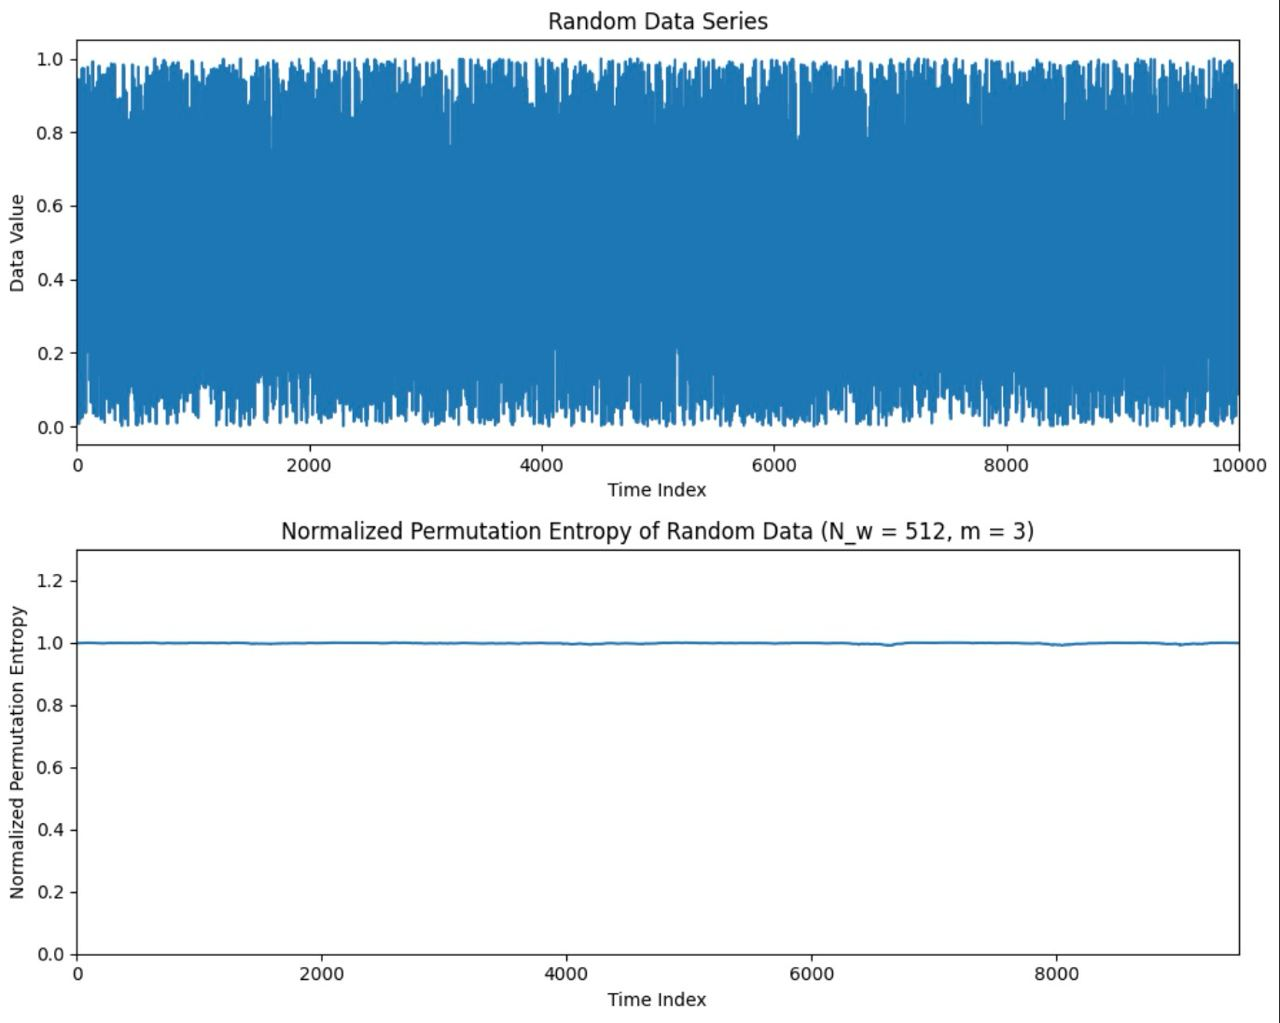
\includegraphics[width=0.5\textwidth]{images/first.jpg}
    \caption{Random data series and corresponding permutation entropy, showing high randomness with entropy near the maximum value.}
\end{figure}
\end{frame}

\begin{frame}{Data Modification: Structured Pattern}
To introduce a structured pattern, the segment between indices \textbf{3000} and \textbf{4000} was partially sorted in chunks of size 20:

\[
x_{i:i+20} = \text{sort}(x_{i:i+20}) \quad \text{for } i \in [3000, 4000]
\]

This reduced the randomness while keeping the mean and variance of the data consistent.
\end{frame}

\begin{frame}{Modified Data Series Plot}
\begin{figure}[ht]
    \centering
    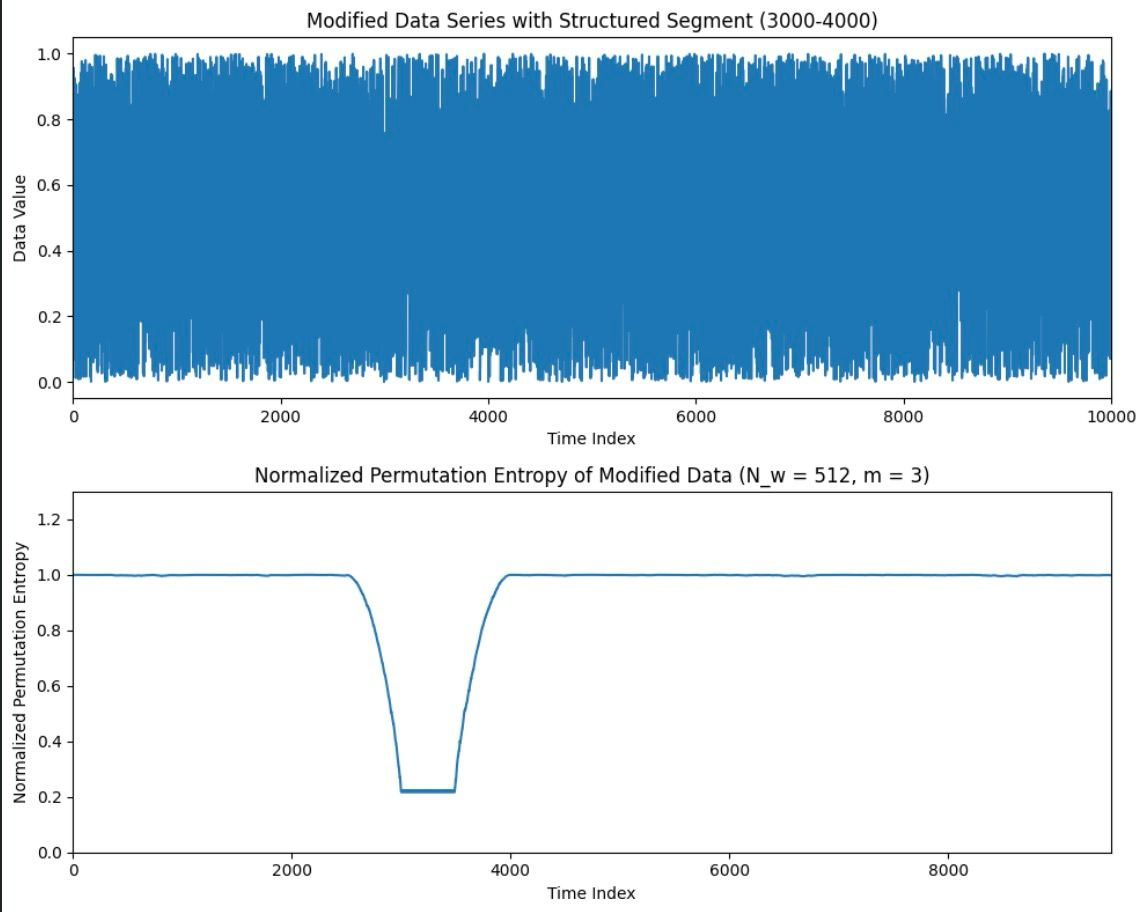
\includegraphics[width=0.5\textwidth]{images/second.jpg}
    \caption{Modified data series with a structured segment (indices 3000 to 4000). The entropy decreases, indicating reduced randomness.}
\end{figure}
\end{frame}

\begin{frame}{Results and Analysis}
For the \textbf{random data series}, the entropy remained close to the theoretical maximum:

\[
H_{\max} = \log_2(m!) = \log_2(6) \approx 2.585
\]

The normalized permutation entropy approached \textbf{1}, implying a high degree of randomness. 

After modifying the segment between indices \textbf{3000} and \textbf{4000}, the entropy dropped due to the partial sorting, indicating reduced randomness in that region:

\[
H' < 1 \quad \text{for the modified region}
\]
\end{frame}

\begin{frame}{Conclusion}
The \textbf{permutation entropy} effectively captured changes in the time series complexity. The random data exhibited entropy near the theoretical maximum, while the structured segment showed a decrease in entropy, indicating the presence of a pattern.

Permutation entropy is useful for detecting complexity changes and can be applied in anomaly detection in more complex datasets.
\end{frame}
